% !TeX encoding = UTF-8
% !TeX spellcheck = pt_BR
% !TeX program = pdflatex
%% ============================================================================
%%  ARTIGO CIENTÍFICO -- TRABALHO DE CONCLUSÃO DE CURSO 2 (TCC 2)
%%  Curso de Engenharia de Computação -- UTFPR Câmpus Apucarana (COENC-AP)
%%
%%  Baseado no modelo oficial do curso (coenc-utfpr.sty). Atende às normas:
%%    ABNT NBR 6022:2018 (artigo científico), NBR 6023:2018 (referências),
%%    NBR 10520:2023 (citações), NBR 6024:2012 (numeração de seções),
%%    NBR 6028:2021 (resumo), IBGE (1993) para tabelas.
%%
%%  COMPILAÇÃO:  pdflatex -> bibtex -> pdflatex -> pdflatex
%%               (ou simplesmente: latexmk -pdf artigo.tex)
%%  As figuras estão na pasta figuras/ (PDF vetorial).
%% ============================================================================
\documentclass[11pt,a4paper]{article}

%% ------------------------- CONFIGURAÇÃO RÁPIDA ------------------------------
\newif\ifduascolunas \duascolunastrue
\newcommand{\idiomaprincipal}{brazilian}

%% ------------------------------ PACOTES -------------------------------------
\usepackage[a4paper,top=3cm,left=3cm,bottom=2cm,right=2cm,
            columnsep=0.7cm,headsep=0.6cm]{geometry}
\usepackage[T1]{fontenc}
\usepackage[utf8]{inputenc}
\usepackage[english,brazilian]{babel} % último = idioma principal
\usepackage{mathptmx}        % fonte Times (recomendação UTFPR: Times ou Arial)
\usepackage{microtype}
\usepackage{amsmath,amssymb}
\usepackage{icomma}          % vírgula decimal correta em fórmulas: 3,14
\usepackage{booktabs,tabularx,multirow,makecell,array}
\usepackage[output-decimal-marker={,},group-separator={.}]{siunitx}
\usepackage[inline]{enumitem}
\usepackage{caption,subcaption}
\usepackage{titlesec}
\usepackage{fancyhdr,lastpage}
\usepackage{indentfirst}
\usepackage[hidelinks]{hyperref}
\usepackage{orcidlink}
\usepackage{xurl}
\usepackage[alf,abnt-opcoes-coenc]{abntex2cite} % citações autor-data ABNT
\usepackage[semdicas]{coenc-utfpr}     % identidade visual (sem caixas de orientação)

%% ---------------------- FORMATAÇÃO CONFORME ABNT ----------------------------
\setlength{\parindent}{1.25cm}
\setlength{\parskip}{0pt}
\setlength{\emergencystretch}{1.5em} % evita linhas que ultrapassam a margem
\setlist{nosep,leftmargin=*}

% Seções (NBR 6024): indicativo numérico sem ponto final, separado do título
\titleformat{\section}{\normalfont\normalsize\bfseries}{\thesection}{0.5em}{\MakeUppercase}
\titleformat{\subsection}{\normalfont\normalsize}{\thesubsection}{0.5em}{\MakeUppercase}
\titleformat{\subsubsection}{\normalfont\normalsize\bfseries}{\thesubsubsection}{0.5em}{}
\titleformat{name=\section,numberless}{\normalfont\normalsize\bfseries\filcenter}{}{0pt}{\MakeUppercase}
\titlespacing*{\section}{0pt}{1.2em}{0.6em}
\titlespacing*{\subsection}{0pt}{0.9em}{0.5em}
\titlespacing*{\subsubsection}{0pt}{0.8em}{0.4em}

% Legendas (NBR 14724): identificação na parte SUPERIOR; fonte na INFERIOR.
\captionsetup{labelsep=endash,font=small,justification=centering,
              skip=4pt,position=top}
\captionsetup[sub]{font=footnotesize}
\DeclareCaptionType[fileext=loq]{quadro}[Quadro][Lista de quadros]
\captionsetup[quadro]{labelsep=endash,font=small,position=top}
\newcommand{\fonte}[1]{\par\vspace{2pt}{\footnotesize Fonte: #1\par}}
\newlength{\recuocitacao}
\ifduascolunas\setlength{\recuocitacao}{2cm}\else\setlength{\recuocitacao}{4cm}\fi
\newenvironment{citacao}{\begin{list}{}{\setlength{\leftmargin}{\recuocitacao}%
  \setlength{\rightmargin}{0pt}\setlength{\topsep}{4pt}}\item[]\footnotesize}%
  {\end{list}}
\newcommand{\nota}[1]{\par{\footnotesize Nota: #1\par}}
\addto\captionsbrazilian{\renewcommand{\tablename}{Tabela}%
  \renewcommand{\figurename}{Figura}\renewcommand{\refname}{Referências}}

% Atalhos de notação usados no texto
\newcommand{\gi}[1]{\ensuremath{#1}\,Gi}
\newcommand{\mi}[1]{\ensuremath{#1}\,Mi}

% Cabeçalho e rodapé
\pagestyle{fancy}
\fancyhf{}
\setlength{\headheight}{14pt}
\fancyhead[L]{\footnotesize\textit{TCC 2 -- \nomecurso{} -- UTFPR \nomecampus}}
\fancyhead[R]{\footnotesize \thepage}
\renewcommand{\headrule}{{\color{utfpramarelo}\hrule height 1pt}}
\fancypagestyle{primeira}{\fancyhf{}\renewcommand{\headrule}{}%
  \fancyfoot[R]{\footnotesize \thepage}}

% Apêndices de artigo: "APÊNDICE A – Título" (NBR 6022)
\newcounter{apendice}
\newcommand{\apendice}[1]{\refstepcounter{apendice}%
  \section*{Apêndice \Alph{apendice} -- #1}}

%% =========================== DADOS DO TRABALHO ==============================
\newcommand{\titulo}{Orquestrador Híbrido com LLM e Decisões Determinísticas para Alocação de Recursos em Sistemas Distribuídos}
\newcommand{\tituloingles}{Hybrid Orchestrator with LLM and Deterministic Decisions for Resource Allocation in Distributed Systems}
\newcommand{\autor}{Lucas Santos Souza}
\newcommand{\orientador}{André Luiz Tinassi D'Amato}
\newcommand{\datadefesa}{\preencher{dd} de \preencher{mês} de \preencher{aaaa}}

\hypersetup{pdftitle={Orquestrador híbrido com LLM e decisões determinísticas -- TCC 2 -- UTFPR-AP},
            pdfauthor={Lucas Santos Souza}}

\begin{document}

%% ======================= ELEMENTOS PRÉ-TEXTUAIS =============================
\newcommand{\primeirapagina}{%
  \cabecalhoinstitucional
  \par\vspace{6pt}
  \noindent\colorbox{utfprpreto}{\parbox{\dimexpr\linewidth-2\fboxsep}{%
    \centering\color{white}\footnotesize\bfseries
    TRABALHO DE CONCLUSÃO DE CURSO 2 \,--\, ARTIGO CIENTÍFICO}}
  \par\vspace{12pt}
  \begin{center}
    {\large\bfseries \titulo\par}
    \vspace{4pt}
    {\normalsize\itshape \tituloingles\par}
    \vspace{10pt}
    {\normalsize \autor\textsuperscript{*}
      \quad \orientador\textsuperscript{**}\par}
    \vspace{3pt}
    {\footnotesize
     \textsuperscript{*}Discente do Curso de Bacharelado em \nomecurso,
       UTFPR, \nomecampus. E-mail: \texttt{lsouza@alunos.utfpr.edu.br}\\
     \textsuperscript{**}Orientador. Docente da \nomecoordenacao,
       UTFPR, \nomecampus. E-mail: \texttt{andredamato@utfpr.edu.br}\par}
  \end{center}
  \vspace{6pt}
  \noindent{\color{utfprcinza}\rule{\linewidth}{0.4pt}}\par\vspace{4pt}
  % --- RESUMO (NBR 6028:2021)
  \noindent{\small\textbf{Resumo:} Ambientes distribuídos com camadas
  \textit{Edge}, \textit{Fog} e \textit{Cloud} reúnem recursos heterogêneos,
  e o escalonador padrão do Kubernetes escolhe o nó apenas pela capacidade
  declarada na submissão, sem usar histórico de execução, telemetria de uso
  ou preferência de camada. Este trabalho propõe um \textit{broker} externo
  ao plano de controle do Kubernetes em que um modelo de linguagem de grande
  porte (\textit{Large Language Model} -- LLM) local interpreta o
  \textit{script} e propõe a especificação da tarefa, enquanto a verificação
  de viabilidade, a admissão e a escolha do nó são feitas por regras
  determinísticas: filtro de recursos, ranqueamento multicritério com pesos
  que priorizam a execução da tarefa e recálculo do ranking no despacho. A
  abordagem foi comparada à submissão direta em quatro experimentos, em um
  \textit{cluster} Kind com três \textit{workers}. Nenhuma das cinco tarefas
  foi alocada ao nó sob estresse, contra duas de cinco na submissão direta; uma
  requisição de memória de \gi{9,45} foi reduzida para \gi{7,57} e executada,
  enquanto a submissão direta permaneceu sem nó atribuído por falta de nós com
  os recursos exigidos; e a correspondência exata entre a camada preferida e a
  camada de execução subiu de $1/9$ para $4/9$. O histórico ativou a margem
  de segurança de $1{,}25\times$ a partir da terceira execução. Os resultados
  indicam a viabilidade da abordagem nos cenários avaliados, como camada
  complementar ao escalonador nativo e não como substituto, sem demonstrar
  otimização global.\par}
  \vspace{4pt}
  \noindent{\small\textbf{Palavras-chave:} Kubernetes; computação em névoa;
  orquestração híbrida; ranqueamento de nós; admissão de recursos.\par}
  \vspace{8pt}
  % --- ABSTRACT
  \noindent{\small\selectlanguage{english}\textbf{Abstract:} Distributed
  environments with Edge, Fog, and Cloud layers gather heterogeneous
  resources, and the default Kubernetes scheduler selects a node only from
  the capacity declared at submission, without using execution history,
  usage telemetry, or layer preference. This work proposes and evaluates a
  broker external to the Kubernetes control plane in which a local Large
  Language Model (LLM) interprets the script and proposes the task
  specification, while feasibility checking, admission, and node selection
  are performed by deterministic rules: resource filtering, multi-criteria
  ranking with weights that prioritize task execution, and ranking
  recomputation at dispatch time. The approach was compared with direct
  submission in four experiments on a Kind cluster with three workers. None
  of the five tasks was placed on the stressed node, against two out of five
  under direct submission; a memory request of 9.45~Gi was reduced to
  7.57~Gi and executed, whereas direct submission remained without an
  assigned node because no node had the required resources; and the exact
  match between the preferred and the execution layer rose from $1/9$ to
  $4/9$. The history activated the $1.25\times$ safety margin from the third
  execution on. The results indicate the feasibility of the approach in the
  evaluated scenarios, as a layer complementary to the native scheduler
  rather than a replacement, without demonstrating global optimization.\par}
  \vspace{4pt}
  \noindent{\small\selectlanguage{english}\textbf{Keywords:} Kubernetes; fog
  computing; hybrid orchestration; node ranking; resource admission.\par}
  \selectlanguage{\idiomaprincipal}
  \vspace{6pt}
  % Data de defesa ainda nao agendada: reativar a linha abaixo quando houver data.
  % \noindent{\footnotesize Data de defesa: \datadefesa.\par}
  \noindent{\color{utfprcinza}\rule{\linewidth}{0.4pt}}\par
  \vspace{10pt}
}

\ifduascolunas
  \twocolumn[\begin{minipage}{\textwidth}\primeirapagina\end{minipage}]
\else
  \primeirapagina
\fi
\thispagestyle{primeira}

%% ============================ 1 INTRODUÇÃO =================================
\section{Introdução}\label{sec:introducao}

A diversidade crescente de aplicações distribuídas, em particular na Internet
das Coisas (\textit{Internet of Things} -- IoT), intensificou o desafio de
alocar recursos computacionais de acordo com cada tarefa e com as condições
da infraestrutura \cite{bonomi2012fog}. Arquiteturas organizadas em camadas \textit{Edge},
\textit{Fog} e \textit{Cloud} distribuem as cargas entre dispositivos de
capacidades distintas, de modo a aproximar o processamento de quem produz os
dados \cite{bonomi2012fog,satyanarayanan2017edge}. A disponibilidade dessas
camadas, porém, não decide por si só onde uma tarefa deve executar nem quais
recursos deve receber. Em ambientes containerizados, essa decisão segue os
requisitos declarados na submissão, embora o comportamento real da tarefa
possa diferir da especificação e execuções anteriores possam informar
dimensionamentos futuros.

O Kubernetes é a plataforma mais difundida para orquestrar contêineres e
descende diretamente da experiência do Borg
\cite{burns2016borg}. Seu escalonador seleciona o nó em duas etapas, filtragem
e pontuação, a partir dos requisitos de recursos declarados no Pod; quando
nenhum nó é viável, o Pod permanece sem nó atribuído.
Esse comportamento nativo não incorpora histórico de execução, telemetria de
uso nem preferência por camada \textit{Edge}/\textit{Fog}/\textit{Cloud} na
decisão, e os requisitos declarados permanecem fixos mesmo quando execuções anteriores evidenciam a necessidade de redimensionamento. Isso motiva mecanismos complementares que combinem
informações históricas, de telemetria e de contexto \textbf{antes} de a
carga de trabalho ser criada.

Modelos de linguagem de grande porte (\textit{Large Language Models} --
LLMs) são candidatos naturais para interpretar o código de uma tarefa e
propor sua especificação, mas delegar a eles a decisão operacional
compromete a previsibilidade e a auditabilidade do despacho. Este trabalho
adota, portanto, uma divisão explícita de responsabilidades: o LLM interpreta
e propõe e as regras determinísticas verificam, admitem e escolhem o nó.

\textbf{Lacuna.} Os trabalhos revisados na Seção~\ref{sec:relacionados}
tratam o escalonamento multirrecurso, a estimativa de demanda a partir de
histórico ou a formação de ambientes \textit{Fog}, mas, entre eles, nenhum
combina, em um componente externo ao escalonador padrão, interpretação
semântica da tarefa por LLM, recalibração por histórico, admissão com regra
explícita para requisições acima da capacidade e decisão final
determinística e auditável.

\textbf{Justificativa.} Requisições subdimensionadas causam estrangulamento
ou falha da tarefa, e requisições acima da capacidade de qualquer nó a deixam
indefinidamente sem nó atribuído, sem que o escalonador nativo use o
histórico de execuções para corrigir nenhuma das duas situações. Tratar esse
problema fora do plano de controle, com decisões registradas e reprodutíveis,
permite avaliar o ganho sem alterar o escalonador padrão, o que é relevante
para ambientes \textit{Edge}/\textit{Fog}/\textit{Cloud}, em que a
heterogeneidade dos nós torna a escolha do local de execução mais sensível.

\textbf{Contribuições.} (i) Uma arquitetura de \textit{broker} externo ao
plano de controle do Kubernetes, com separação explícita entre o que o LLM
faz e o que as regras decidem; (ii) um ranqueador de nós determinístico e
reprodutível (NodeRanker), recalculado no despacho; (iii) uma regra de
admissão \textit{best-effort} que evita Pods sem nó atribuído dentro de uma
janela de $80\%$; e (iv) uma avaliação experimental em quatro cenários, com
os registros completos de execução (\textit{logs}) preservados.

\textbf{Organização.} A Seção~\ref{sec:fundamentacao} apresenta a
fundamentação; a Seção~\ref{sec:relacionados} compara criticamente os
trabalhos relacionados; a Seção~\ref{sec:metodos} descreve a arquitetura, o
papel do LLM e o protocolo experimental; a Seção~\ref{sec:resultados} traz os
resultados e a discussão; e a Seção~\ref{sec:conclusao} conclui e propõe
trabalhos futuros.

\subsection{Objetivos}\label{sec:objetivos}

O objetivo geral é propor e avaliar um \textit{broker} externo ao plano de
controle do Kubernetes que combine um LLM local, para interpretar a tarefa e
propor sua especificação, com mecanismos determinísticos para verificar a
viabilidade dos recursos e selecionar o nó de execução. Os objetivos
específicos são:
\begin{enumerate}[label=\alph*)]
  \item projetar a arquitetura do \textit{broker}, separando as funções do
        LLM das decisões determinísticas;
  \item implementar o NodeRanker e a regra de admissão
        \textit{best-effort};
  \item avaliar, em quatro experimentos controlados, a recalibração por
        histórico, a seleção sob nó sobrecarregado, o tratamento de
        requisições acima da capacidade e a afinidade de camada; 
  \item registrar e disponibilizar os \textit{logs} de cada execução para
        auditoria e reprodução.
\end{enumerate}

%% ===================== 2 FUNDAMENTAÇÃO TEÓRICA ============================
\section{Fundamentação teórica}\label{sec:fundamentacao}

\subsection{Computação \textit{Edge}, \textit{Fog} e \textit{Cloud}}

A computação em névoa (\textit{fog computing}) estende o modelo da nuvem para
a borda da rede e se caracteriza por baixa latência, distribuição geográfica
ampla e heterogeneidade de nós \cite{bonomi2012fog}. A computação de borda
(\textit{edge computing}) posiciona recursos próximos dos dispositivos
móveis e sensores, reduzindo a dependência de um \textit{datacenter} remoto
\cite{satyanarayanan2017edge}. Neste trabalho, as camadas \textit{Edge},
\textit{Fog} e \textit{Cloud} são tratadas como rótulos de nós, usados como
preferência de posicionamento.

A computação em nuvem (\textit{cloud computing}), por sua vez, concentra
grande capacidade de processamento e armazenamento em \textit{datacenters}
remotos, com alta capacidade e maior latência até quem produz os dados. As três
camadas formam um \textit{continuum} em que a capacidade cresce da borda para a
nuvem e a latência cresce no mesmo sentido, de modo que decidir onde uma tarefa
executa é um compromisso entre os dois fatores. A orquestração nesse
\textit{continuum} é tratada na literatura como um problema aberto de
gerenciamento de recursos heterogêneos e dinâmicos \cite{ullah2023continuum}, o
que justifica um componente que combine contexto da tarefa e do ambiente antes
da alocação.

\subsection{Escalonamento no Kubernetes}

O Kubernetes é uma plataforma de orquestração de contêineres, descendente do
Borg \cite{verma2015borg}, em que a unidade de execução é o Pod, um conjunto de
contêineres escalonado em conjunto, e uma tarefa finita é descrita por um
recurso do tipo Job, que cria Pods até a conclusão. Cada Pod declara a
quantidade de CPU e de memória que \textit{solicita} (\textit{requests}) e o
máximo que pode consumir (\textit{limits}).

O \textit{kube-scheduler} é o componente do plano de controle que decide em
qual nó cada Pod ainda sem nó será executado \cite{k8s2026scheduler}. Ele
opera em duas etapas. Na filtragem, descartam-se os nós que não comportam o
Pod, por exemplo porque a soma dos \textit{requests} já alocados mais o do novo
Pod excederia a capacidade alocável do nó, ou porque o Pod restringe o nó por
rótulo. Na pontuação, os nós restantes recebem notas de \textit{plugins}, como
o balanceamento de recursos alocados e a presença local da imagem do
contêiner, e o de maior nota é escolhido. Se nenhum nó passa na filtragem, o
Pod permanece na fase \textit{Pending}, com o evento de falha de
escalonamento, até que algum nó passe a comportá-lo.

Esse mecanismo é relevante para o problema tratado por duas razões. A
primeira é que a filtragem compara \textit{requests} declarados com a
capacidade alocável, e não com a utilização observada, de modo que um nó
saturado pode continuar elegível e um valor declarado a menos ou a mais não é
corrigido por execuções anteriores. A segunda é que uma requisição acima da
capacidade de todos os nós nunca é atendida, o que motiva a regra de admissão
descrita na Seção~\ref{sec:metodos}. Como o \textit{broker} proposto fixa o
nó escolhido por rótulo de nome, a filtragem do \textit{kube-scheduler}
continua valendo, e é nela que a requisição é finalmente aceita ou barrada.

\subsection{Alocação multirrecurso e uso de histórico}

A alocação multirrecurso consiste na distribuição coordenada de cargas de
trabalho que disputam simultaneamente diferentes dimensões computacionais,
como processamento, memória e rede. Para otimizar esse processo, o sistema
Tetris \cite{grandl2014tetris} modela as demandas das tarefas e as
capacidades disponíveis dos nós como vetores, priorizando alocações que
maximizam o alinhamento entre oferta e demanda para reduzir a fragmentação de
recursos. Esse conceito é diretamente relevante para o presente trabalho por
fundamentar a avaliação conjunta de múltiplas métricas na etapa de pontuação
dos nós; entretanto, o modelo pressupõe que os requisitos de cada tarefa já
sejam conhecidos e exatos no momento da submissão.

Por sua vez, a estimativa de demanda baseada em histórico busca inferir a
real necessidade computacional de uma aplicação a partir de dados empíricos,
reduzindo a dependência de configurações manuais estáticas. Nesse contexto, o
Quasar \cite{delimitrou2014quasar} utiliza técnicas de classificação para
estimar o perfil de desempenho e de interferência de novas cargas por
comparação com execuções conhecidas, enquanto o Autopilot
\cite{rzadca2020autopilot} analisa séries históricas de consumo observado
para ajustar automaticamente os limites de CPU e memória ao longo do tempo.
Esses mecanismos embasam o uso de registros históricos no \textit{broker}
proposto para calibrar requisições recorrentes. Contudo, por operarem
exclusivamente sobre sinais quantitativos e telemetria observada, tais
abordagens não realizam a interpretação semântica do código-fonte da tarefa
para antecipar seu comportamento antes da primeira execução.

\subsection{LLM local e temperatura de amostragem}

Um LLM gera texto escolhendo, a cada passo, o próximo \textit{token} a partir
de uma distribuição de probabilidades. A \textit{temperatura} controla a
aleatoriedade dessa escolha: valores maiores espalham a probabilidade entre
mais \textit{tokens}, e o valor zero faz o modelo tender a escolher sempre o
\textit{token} mais provável. Servidores locais como o Ollama
\cite{ollama2026} expõem esse parâmetro.

\citeonline{renze2024temperature} investigaram empiricamente se a temperatura
afeta o desempenho de LLMs na resolução de problemas. O estudo montou provas
de múltipla escolha a partir de problemas sorteados de \textit{benchmarks}
padronizados, avaliou nove LLMs combinados com cinco técnicas de elaboração de
\textit{prompts} e variou a temperatura de $0{,}0$ a $1{,}6$. Os autores
concluíram que variações entre $0{,}0$ e $1{,}0$ não têm impacto
estatisticamente significativo no desempenho, resultado que se manteve entre
modelos, técnicas de \textit{prompt} e domínios de problema. Isso é útil ao
presente trabalho porque indica que fixar a temperatura em $0$, escolha que
favorece a reprodutibilidade da especificação gerada, não deve custar acerto
nas respostas. A evidência é, porém, indireta: as tarefas avaliadas são de
múltipla escolha, não está claro que o resultado valha para um modelo pequeno
como o usado aqui, e nenhuma delas produz saída estruturada para planejamento
de infraestrutura.
Por isso, a escolha foi verificada em uma análise própria
(Seção~\ref{sec:temperatura}).

%% ===================== 3 TRABALHOS RELACIONADOS ===========================
\section{Trabalhos relacionados}\label{sec:relacionados}

Esta seção analisa abordagens da literatura sobre escalonamento adaptativo e
alocação de recursos em ambientes distribuídos, agrupadas em três eixos. Os
trabalhos foram selecionados por tratarem de (i) escalonamento e
admissão de recursos em \textit{clusters}, (ii) estimativa de demanda por
histórico ou aprendizado, ou (iii) alocação em ambientes \textit{Fog}. O
Quadro~\ref{qua:relacionados} compara-os segundo critérios que importam ao
problema aqui tratado: técnica empregada, nível de atuação (substitui ou
complementa o escalonador) e limitação frente a este trabalho.

A busca incluiu artigos, trabalhos de conclusão de curso, trabalhos
acadêmicos e livros, nas bases SciELO, Scholarpedia, Minha Biblioteca e Google
Acadêmico, além de indicações do orientador.
Os termos de busca combinaram \textit{fog computing}, computação de borda,
orquestração de contêineres, Kubernetes, alocação dinâmica de recursos,
\textit{task offloading}, classificação de tarefas e modelos de linguagem
aplicados a Kubernetes. Obras clássicas de orquestração em larga escala e de
sistemas distribuídos foram mantidas por constituírem a base conceitual da
área, sendo complementadas por estudos recentes sobre escalonamento
customizado, orquestração no \textit{continuum} \textit{Edge}--\textit{Cloud}
e LLMs.

\begin{quadro*}[t]
  \caption{Comparação crítica entre trabalhos relacionados.}
  \label{qua:relacionados}
  \centering\footnotesize
  \setlength{\tabcolsep}{3pt}
  \begin{tabularx}{\linewidth}{|>{\raggedright\arraybackslash}p{3.6cm}|>{\raggedright\arraybackslash}X|>{\raggedright\arraybackslash}X|}
    \hline
    \textbf{Trabalho} & \textbf{Abordagem} & \textbf{Limitação frente a este trabalho}\\ \hline
    \citeonline{verma2015borg}; \citeonline{burns2016borg} &
      Controle de admissão e empacotamento sobre recursos declarados &
      Decide pela capacidade pedida; sem histórico nem preferência de
      camada; Pod fica sem nó se nada cabe\\ \hline
    \citeonline{gog2016firmament} &
      Escalonador centralizado por fluxo de custo mínimo sobre o estado
      global &
      Substitui o escalonador; não infere nem recalibra a especificação da
      tarefa\\ \hline
    \citeonline{grandl2014tetris} &
      Empacotamento multirrecurso de tarefas &
      Opera sobre as demandas de cada tarefa; sem interpretação da
      tarefa por LLM nem camadas \textit{Fog}\\ \hline
    \citeonline{delimitrou2014quasar} &
      Gestão ciente de qualidade de serviço (\textit{Quality of Service} --
      QoS) com estimativa de necessidades &
      Estimativa quantitativa; sem camadas \textit{Edge}/\textit{Fog}/\textit{Cloud}\\ \hline
    \citeonline{rzadca2020autopilot} &
      Ajuste automático de recursos de jobs com base no uso &
      Ajusta limites; não escolhe nó nem usa preferência topológica\\ \hline
    \citeonline{tao2017nscd} &
      Alocação de contêineres por estado de recursos e inferência
      \textit{fuzzy} &
      Foco no estado de recursos dos nós; sem histórico, preferência de camada
      nem interpretação da tarefa por LLM\\ \hline
    \citeonline{kratzke2024prompt} &
      LLMs geram manifestos Kubernetes por \textit{prompts} (\textit{zero-shot},
      \textit{few-shot} e encadeamento), sem treinamento &
      O manifesto gerado pode exigir intervenção manual; sem filtro
      determinístico de admissão, histórico nem escolha de nó\\ \hline
    \citeonline{rahbari2020offloading} &
      Decisão de \textit{offloading} de módulos em \textit{fog} móvel por
      árvore de classificação e regressão &
      Decide entre dispositivo, \textit{fog} e nuvem em simulação; não atua
      sobre o escalonador do Kubernetes nem dimensiona recursos\\ \hline
    \citeonline{sami2020ondemand}; \citeonline{sami2020fscaler} &
      Formação de \textit{Fog} sob demanda; escalonamento horizontal por
      aprendizado por reforço (\textit{Reinforcement Learning} -- RL) em
      \textit{clusters} \textit{Fog} &
      Foco em formação de \textit{Fog} e escala de instâncias, não em
      admissão; o FScaler usa política aprendida, menos auditável\\ \hline
    \citeonline{li2024tpds}; \citeonline{li2024offline} &
      RL distribucional e RL \textit{offline} para escalonamento de jobs &
      Exigem treinamento de política; não interpretam a tarefa\\ \hline
    \textbf{Este trabalho} &
      LLM local interpreta a tarefa; regras determinísticas admitem e
      escolhem o nó; histórico recalibra a especificação &
      Validação inicial em \textit{cluster} único; sem comparação
      experimental direta com os demais\\ \hline
  \end{tabularx}
  \fonte{Elaborado pelo autor (2026).}
\end{quadro*}

Os escalonadores de \textit{clusters} em larga escala
\cite{verma2015borg,gog2016firmament,grandl2014tetris}
otimizam o empacotamento sobre demandas conhecidas ou declaradas; este
trabalho preserva o escalonador padrão como mecanismo de execução e
acrescenta uma etapa anterior de análise e decisão, em vez de substituí-lo. Os
sistemas que estimam demanda \cite{delimitrou2014quasar,rzadca2020autopilot}
fazem-no de forma quantitativa a partir de medições; aqui, o histórico apenas
recalibra o piso de recursos da execução seguinte, e a interpretação
semântica do \textit{script} fica a cargo do LLM. As abordagens de
aprendizado por reforço
\cite{sami2020fscaler,li2024tpds,li2024offline} aprendem uma política de
escalonamento; o NodeRanker, em contraste, aplica um filtro de viabilidade e
uma pontuação linear cujo cálculo é reproduzível e registrado, ao custo de
pesos definidos manualmente (Seção~\ref{sec:ranker}). Os trabalhos que
selecionam o nó pela carga monitorada
\cite{tao2017nscd} e os que decidem o posicionamento por classificação
\cite{rahbari2020offloading} compartilham com este a ideia de ranquear nós,
mas não usam o histórico nem o perfil semântico da tarefa e, no segundo caso,
a avaliação é simulada. O levantamento de \citeonline{rejiba2022custom}
classifica os escalonadores customizados do Kubernetes por objetivo e por tipo
de carga, e aponta, entre as lacunas, avaliações em \textit{clusters}
pequenos, o que também limita este trabalho. Quanto ao uso de LLMs,
\citeonline{kratzke2024prompt} mostram que modelos de linguagem podem gerar
manifestos Kubernetes apenas com \textit{prompts}, com graus variados de
intervenção manual; aqui, o LLM propõe a especificação, mas ela é validada por
regras antes de ser usada e a escolha do nó não é delegada a ele.

Quanto ao ambiente \textit{Fog}, \citeonline{sami2020ondemand} formam
ambientes de névoa sob demanda: dispositivos voluntários entram na névoa,
gerenciados por um cluster Kubernetes criado com o Kubeadm, e um algoritmo
memético evolutivo escolhe quais voluntários recebem cada serviço, cujos
requisitos de recursos são conhecidos de antemão. Neste trabalho, o papel
equivalente à entrada de dispositivos é cumprido pelo \texttt{node\_agent},
um agente leve em Python executado em cada dispositivo que se registra no
servidor de contexto do \textit{broker} com suas capacidades totais, renova o
registro periodicamente (\textit{heartbeat}, a cada $30$\,s) e expõe um ponto de
consulta de uso atual de CPU, memória e disco, lido sob demanda no momento da
alocação para evitar monitoramento contínuo de todos os nós. A diferença é que
o \texttt{node\_agent} apenas informa o estado dos nós, enquanto a escolha do
nó e o dimensionamento da tarefa cabem ao NodeRanker e às regras de admissão,
e o requisito de recursos não é suposto conhecido, mas proposto pelo LLM e
recalibrado pelo histórico.

\textbf{Lacuna ocupada.} Entre os trabalhos analisados, nenhum une, em um
componente externo ao escalonador padrão, LLM para interpretação da tarefa,
admissão por regra explícita de oversize e decisão final determinística. A
ressalva é que não houve comparação experimental com esses sistemas, de modo
que a contribuição é arquitetural e demonstrada em cenários controlados.

%% ======================= 4 MATERIAIS E MÉTODOS =============================
\section{Materiais e métodos}\label{sec:metodos}

A pesquisa é aplicada e experimental: um protótipo foi implementado e
comparado a uma linha de base em cenários controlados, com a mesma tarefa,
imagem e \textit{cluster} nas duas configurações, de modo que apenas a decisão de
recursos e de alocação varie.

\subsection{Arquitetura da solução}

O \textit{broker} é inserido no fluxo convencional de Jobs do Kubernetes. Na
submissão direta, a requisição chega ao servidor de API e o
\textit{kube-scheduler} seleciona o nó. Na abordagem com \textit{broker}, a
requisição é antes analisada, o histórico é consultado, o estado dos nós é
considerado e a especificação é preparada, de modo que a decisão de alocação
precede a criação do Job sem substituir o plano de controle. A
Figura~\ref{fig:arch} mostra os dois caminhos convergindo para o mesmo
\textit{cluster}.

\begin{figure*}[t]
  \caption{Visão geral dos dois caminhos de execução.}
  \label{fig:arch}
  \centering
  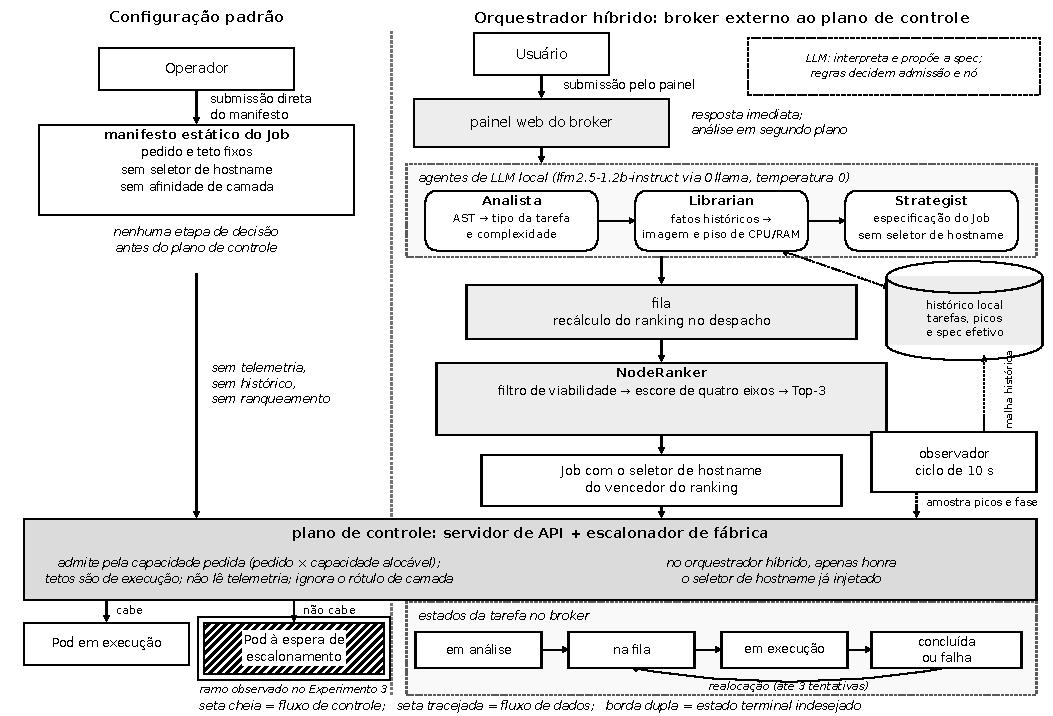
\includegraphics[width=0.85\textwidth]{figuras/fig_arch_dois_canais.pdf}
  \fonte{Elaborado pelo autor (2026).}
\end{figure*}

Um \textit{script} enviado pela interface web é armazenado em SQLite e
processado em segundo plano. Três agentes LLM, descritos na
Seção~\ref{sec:llm}, operam em sequência e produzem a especificação do Job.
A tarefa entra então na fila do \textit{broker}, onde o NodeRanker ranqueia
os nós elegíveis. O ranking do planejamento é apenas uma referência, antes do
despacho os nós são consultados de novo e o ranking é recalculado com
telemetria atualizada. O nó mais bem ranqueado é vinculado à especificação
por um seletor de \textit{hostname} e o Job é submetido; se nenhum nó for
elegível, a tarefa permanece na fila. Durante a execução, um monitor
acompanha os Pods e registra os picos de uso; ao término, picos e
especificação efetiva são gravados no histórico, fechando o ciclo de
realimentação. Em caso de falha ou de estado pendente prolongado, a tarefa
pode retornar à fila excluindo o \textit{hostname} anterior (até três
tentativas).

\subsection{Papel do LLM e escolha da temperatura}\label{sec:llm}

O LLM é um \textbf{interpretador e redator de especificações}, transforma
um \textit{script} não estruturado em uma especificação estruturada de Job.
Ele \textbf{não} escolhe o nó, não decide a admissão e não define a camada
preferida. O modelo usado é o \texttt{LiquidAI/lfm2.5-1.2b-instruct}, com
cerca de $1{,}2$ bilhão de parâmetros, servido localmente via Ollama. Três
agentes operam em sequência, cada um com saída em JSON validada pelo
\textit{broker}:
\begin{enumerate}[label=\alph*)]
  \item o \textbf{Analista} recebe o \textit{script} e as bibliotecas
        extraídas por Árvore Sintática Abstrata (AST) e devolve o tipo da
        tarefa (CPU-bound, IO-bound ou ML-heavy), uma complexidade de $1$ a
        $10$, as bibliotecas e os pacotes necessários;
  \item o \textbf{Librarian} recebe fatos do histórico (telemetria agregada,
        taxa de sucesso por imagem, sinais de que o pico se aproximou do
        limite) e propõe a imagem de contêiner e o piso de CPU e memória;
  \item o \textbf{Strategist} consolida as saídas anteriores em uma
        especificação de Job (\textit{requests}, \textit{limits}, imagem,
        dependências), sem preencher seletor de nó.
\end{enumerate}

Os três tipos de tarefa descrevem o fator que mais limita a execução do
\textit{script}. Uma tarefa \textbf{CPU-bound} é limitada pelo processador,
com laços e cálculos numéricos e pouca espera por dados. Uma tarefa
\textbf{IO-bound} passa a maior parte do tempo esperando entrada e saída, como
leitura e escrita de arquivos ou acesso à rede, e usa pouca CPU. Uma tarefa
\textbf{ML-heavy} realiza treinamento ou inferência de aprendizado de
máquina; o \textit{prompt} do Analista a restringe a \textit{scripts} que
importam explicitamente bibliotecas como \texttt{tensorflow},
\texttt{torch}, \texttt{keras} ou \texttt{sklearn}, e \textit{scripts}
triviais devem ser classificados como CPU-bound ou IO-bound com complexidade
de $1$ a $3$. Esse tipo, junto com a complexidade e os recursos
requisitados, alimenta a regra determinística que define a camada preferida
(Quadro~\ref{qua:camada}), aplicada na ordem do quadro: a primeira condição
satisfeita decide.

\begin{quadro}[h]
  \caption{Regra de camada preferida a partir do perfil da tarefa.}
  \label{qua:camada}
  \centering\footnotesize
  \setlength{\tabcolsep}{3pt}
  \begin{tabularx}{\linewidth}{|>{\raggedright\arraybackslash}p{1.5cm}|>{\raggedright\arraybackslash}X|}
    \hline
    \textbf{Camada} & \textbf{Condição (a primeira satisfeita decide)}\\ \hline
    \textit{Cloud} & tipo ML-heavy; ou complexidade $\geq 8$; ou memória
      $\geq\gi{4}$; ou CPU $\geq 4$ núcleos\\ \hline
    \textit{Fog} & complexidade $\geq 5$; ou tipo CPU-bound; ou memória
      $\geq\gi{1{,}5}$; ou CPU $\geq 2$ núcleos\\ \hline
    \textit{Edge} & nenhuma das anteriores (por exemplo, tarefa IO-bound
      leve)\\ \hline
  \end{tabularx}
  \fonte{Elaborado pelo autor (2026).}
\end{quadro}

Cada saída do LLM passa por validação determinística antes de ser usada: a
imagem deve pertencer ao catálogo permitido, o piso nunca fica abaixo do
mínimo da imagem, a CPU é limitada ao intervalo de $1$ a $8$ núcleos e a
memória a \gi{0,25} a \gi{8} no planejamento. O Quadro~\ref{qua:papeis}
resume a divisão de responsabilidades.

\begin{quadro}[h]
  \caption{Divisão de responsabilidades entre o LLM e as regras determinísticas.}
  \label{qua:papeis}
  \centering\footnotesize
  \setlength{\tabcolsep}{3pt}
  \begin{tabularx}{\linewidth}{|>{\raggedright\arraybackslash}p{2.3cm}|>{\raggedright\arraybackslash}p{1.6cm}|>{\raggedright\arraybackslash}X|}
    \hline
    \textbf{Etapa} & \textbf{Executor} & \textbf{Função}\\ \hline
    Perfil da tarefa & LLM (Analista) & Classifica tipo e complexidade a
      partir do código\\ \hline
    Imagem e piso de recursos & LLM (Librarian) + regras & Propõe; regras
      impõem catálogo, mínimos e margem de $1{,}25\times$\\ \hline
    Especificação do Job & LLM (Strategist) + regras & Consolida
      \textit{requests}/\textit{limits}; regras limitam intervalos\\ \hline
    Camada preferida & Regra & Função determinística do tipo,
      complexidade e recursos\\ \hline
    Viabilidade e admissão & Regra & Filtro de recursos e janela de
      $80\%$\\ \hline
    Escolha do nó & NodeRanker & Pontuação de quatro eixos; recálculo no
      despacho\\ \hline
    Vinculação ao nó & Regra & Seletor de \textit{hostname} do vencedor\\ \hline
  \end{tabularx}
  \fonte{Elaborado pelo autor (2026).}
\end{quadro}

\textbf{Temperatura zero.} Os três agentes usam temperatura $0$. A escolha
foi uma decisão de projeto, com três motivos: (i) a saída é JSON estruturado
consumido por um \textit{parser} e por validadores, e a decodificação
quase determinística tende a reduzir respostas malformadas; (ii) a tarefa é
classificar e extrair, não gerar texto criativo, de modo que diversidade de
amostragem não traz ganho; e (iii) a reprodutibilidade facilita comparar a
especificação gerada entre execuções e auditar o planejamento. A escolha
foi verificada em uma análise de sensibilidade, que compara as
respostas do Analista e do Strategist em temperaturas $0$, $0{,}5$ e $1{,}0$
(Seção~\ref{sec:temperatura}).

\subsection{NodeRanker e justificativa dos pesos}\label{sec:ranker}

Para cada \textit{worker}, o \textit{broker} calcula os recursos efetivos a
partir da capacidade disponível e das reservas registradas; sem telemetria
atualizada, assume metade da capacidade alocável. Um filtro de viabilidade
remove nós com CPU, memória ou disco (quando solicitado) insuficientes. Os
nós restantes recebem a pontuação
\begin{equation}
  S_i = 40\,r_i + 25\,w_i + 15\,d_i + 20\,\ell_i,
  \label{eq:noderanker}
\end{equation}
em que $r_i$ é a adequação de recursos do nó $i$, $w_i$ sua localidade de
imagem, $d_i$ sua folga de disco e $\ell_i$ a afinidade entre sua camada e a
preferência da tarefa, cada termo normalizado em $[0,1]$. O termo de recursos
compara a utilização de CPU e memória de cada candidato com a média dos
candidatos; a localidade de imagem favorece nós que já executaram a imagem; a
afinidade dá a pontuação máxima à camada exata, metade à adjacente e zero à
oposta, sendo neutra sem preferência. Os três melhores candidatos são
registrados para auditoria (Figura~\ref{fig:ranker}).

\textbf{Justificativa dos pesos.} Os pesos foram definidos manualmente para
\textbf{priorizar a execução da tarefa}. O maior peso ($40$) recai sobre a
adequação de recursos, porque é ela que determina se a tarefa executa sem
contenção; a localidade de imagem ($25$) vem a seguir por reduzir o atraso
até o início da execução; a folga de disco ($15$) atua como proteção, já que
a viabilidade mínima é garantida pelo filtro; e a afinidade de camada ($20$)
expressa uma preferência topológica e não uma restrição, de modo que
condições de execução desfavoráveis podem superá-la. Esses valores não foram
calibrados experimentalmente nem submetidos a análise de sensibilidade;
essa análise é apresentada como trabalho futuro (Seção~\ref{sec:conclusao}).

\begin{figure}[t]
  \caption{Pipeline de decisão da fila.}
  \label{fig:ranker}
  \centering
  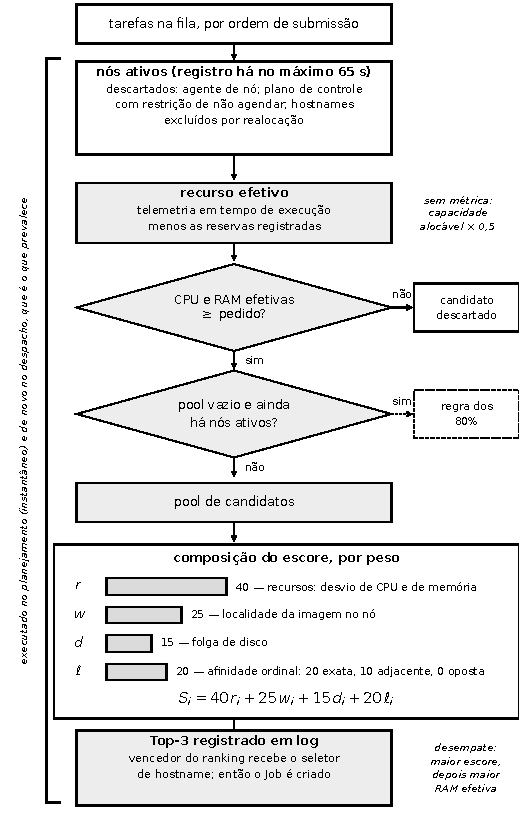
\includegraphics[width=\linewidth]{figuras/fig_noderanker_pipeline.pdf}
  \fonte{Elaborado pelo autor (2026).}
\end{figure}

\subsection{Admissão \textit{best-effort} e realimentação}

Quando nenhum nó satisfaz integralmente a requisição, o \textit{broker}
calcula a CPU e a memória efetivas máximas entre os \textit{workers} ativos,
$R_{\max}^{\mathrm{cpu}}$ e $R_{\max}^{\mathrm{mem}}$. A admissão só se aplica
se ao menos $80\%$ de cada recurso requisitado estiver disponível; caso
contrário, a tarefa permanece na fila e nenhum Pod é criado. Do contrário,
cada recurso é ajustado de forma independente, conforme a
Equação~\eqref{eq:clamp}:
\begin{equation}
  \begin{split}
    R'^{x}&=\max\bigl(0{,}80\,R^{x},\;\min(R^{x},R_{\max}^{x})\bigr),\\
    &x\in\{\mathrm{cpu},\mathrm{mem}\}.
  \end{split}
  \label{eq:clamp}
\end{equation}
O valor ajustado é usado na requisição e no limite, e o ajuste é registrado
nos metadados de despacho. A Figura~\ref{fig:clamp} ilustra as três regiões
para a memória. Para a realimentação, quando o histórico indica que uma
execução se aproximou do limite alocado (pico $\geq 85\%$), o Librarian
aplica uma margem de $1{,}25\times$ sobre o piso, limitada a $2{,}0\times$.

Em termos práticos, \textit{best-effort} (``melhor esforço'') significa
executar a tarefa com menos recursos do que o solicitado, em vez de recusá-la,
desde que a redução seja pequena. A requisição é reduzida até o maior valor
que algum nó consegue oferecer, e nunca abaixo de $80\%$ do valor original;
reduções maiores que $20\%$ são recusadas, porque a execução com recursos
muito aquém do pedido tende a falhar por falta de memória. Duas
consequências decorrem da regra. A primeira é que a requisição só é admitida
se $R_{\max}\geq 0{,}80\,R$, ou seja, se $R\leq R_{\max}/0{,}80=1{,}25\,R_{\max}$,
o que define o teto da janela de admissão. A segunda é que a admissão não
garante o sucesso da execução, apenas evita que a tarefa fique parada na
fila quando falta pouco para que ela caiba. Por exemplo, com
$R_{\max}=\gi{7,5}$ de memória, um pedido de \gi{8} seria reduzido para
\gi{7,5} ($93{,}75\%$ do pedido), enquanto um pedido de \gi{10} permaneceria
na fila, pois $0{,}80\times 10=\gi{8}>R_{\max}$. O Kubernetes, por si só, não
faz essa redução: o Pod com requisição superior à capacidade de qualquer nó
permanece em \textit{Pending}.

\begin{figure}[t]
  \caption{Regra dos $80\%$ para admissão \textit{best-effort} na memória.}
  \label{fig:clamp}
  \centering
  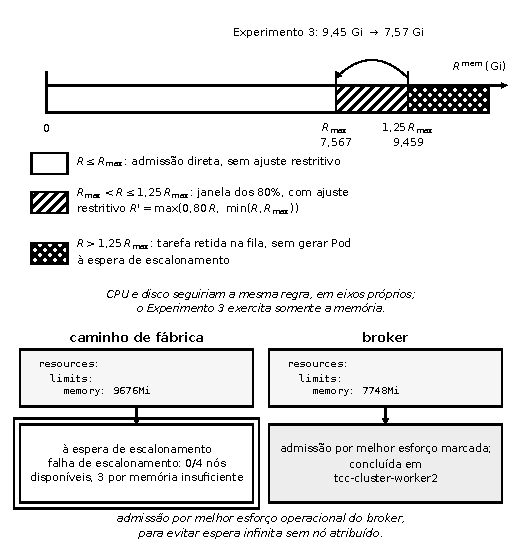
\includegraphics[width=\linewidth]{figuras/fig_regra_80.pdf}
  \fonte{Elaborado pelo autor (2026).}
\end{figure}

\subsection{Materiais}

Todas as quantidades de memória usam as unidades do Kubernetes, em base
binária: \textit{gibibyte} (Gi, $2^{30}$ bytes) e \textit{mebibyte} (Mi,
$2^{20}$ bytes), de modo que $1$\,Gi $=1024$\,Mi. O ambiente está resumido na
Tabela~\ref{tab:materiais}. O \textit{cluster}
foi criado com Kind, os doi métodos não executaram
simultaneamente e a semente de amostragem do modelo não foi fixada.

\begin{table}[t]
  \caption{Ambiente experimental utilizado.}
  \label{tab:materiais}
  \centering\footnotesize
  \begin{tabular}{@{}p{2.6cm}p{4.6cm}@{}}
    \toprule
    Item & Especificação\\
    \midrule
    Hospedeiro & AMD Ryzen 5 3600X (6 núcleos, 12 \textit{threads}),
      \gi{16,0} de RAM, Windows 11 Pro, Docker 28.2.2\\
    \textit{Cluster} & Kind, Kubernetes v1.32.2: 1 plano de controle e 3
      \textit{workers} de \gi{7,716} alocáveis, rotulados \textit{edge},
      \textit{fog} e \textit{cloud}\\
    Telemetria & Metrics Server v0.8.1\\
    LLM & \texttt{lfm2.5-1.2b-instruct} via Ollama, temperatura $0$\\
    \textit{Broker} & Python 3.11, SQLite\\
    Imagem de tarefa & \texttt{python:3.11-slim}\\
    \bottomrule
  \end{tabular}
  \fonte{Elaborado pelo autor (2026).}
\end{table}

\subsection{Avaliação}

Cada um dos quatro experimentos compara a submissão direta (configuração padrão)
com a submissão via \textit{broker}. O \textbf{Exp.~1} executa a mesma
tarefa dez vezes em sequência; a submissão direta mantém requisição e limite
de memória fixos em \mi{256}, e no \textit{broker} a primeira execução não
tem histórico. A métrica é a folga $\Delta RAM$, calculada pela
Equação~\eqref{eq:delta_ram},
\begin{equation}
  \Delta RAM = RAM_{\mathrm{limit}} - RAM_{\mathrm{peak}},
  \label{eq:delta_ram}
\end{equation}
em que $RAM_{\mathrm{limit}}$ é o limite efetivo de memória e
$RAM_{\mathrm{peak}}$ o pico observado. O \textbf{Exp.~2} submete cinco tarefas idênticas em rajada enquanto um processo de
estresse, com requisições modestas que mantêm o nó elegível, executa no
\textit{worker} \textit{fog}; conta-se quantas tarefas vão ao nó
estressado, e a corrida só é válida se o nó apresentar CPU elevada (acima de
$500$\,m) após o aquecimento. O \textbf{Exp.~3} submete uma requisição
acima da capacidade efetiva, \textbf{idêntica nos dois modelos}: \gi{9,45}
(\mi{9676}), valor escolhido por pertencer à janela $(R_{\max}, 1{,}25R_{\max}]$
e, portanto, exceder a capacidade de todos os nós sem ultrapassar o limite da
regra de $80\%$. O \textbf{Exp.~4} executa nove tarefas (três para cada camada) alternando as
preferências \textit{edge}, \textit{fog} e \textit{cloud}, com a imagem
pré-carregada nos \textit{workers}; a métrica é a correspondência entre
camada preferida e camada de execução. As amostras são pequenas e cada cenário foi executado uma vez por modelo, de modo
que os resultados são apresentados como contagens e séries, sem média e
desvio padrão entre repetições do cenário completo.

\subsection{Disponibilidade do código e dos dados}

Os \textit{scripts} dos experimentos (\texttt{scripts/\allowbreak run\_\allowbreak exp*}) e os
registros completos de cada execução (\textit{logs} do console, saída do
\texttt{kubectl describe} e linhas de log do \textit{broker}, em
\texttt{results/\allowbreak metrics\_\allowbreak export/\allowbreak exp*/\allowbreak logs}) acompanham o código-fonte do
projeto, disponível em \preencher{URL do repositório}, sob licença
\preencher{MIT, ou a definida com o orientador}, na versão
\preencher{tag da versão}. As versões exatas do ambiente estão na
Tabela~\ref{tab:materiais}; nenhuma credencial ou dado pessoal compõe os
registros.

%% ===================== 5 RESULTADOS E DISCUSSÃO ===========================
\section{Resultados e discussão}\label{sec:resultados}

A Tabela~\ref{tab:resumo} sintetiza os quatro experimentos. As subseções
seguintes detalham cada um.

\begin{table}[h]
  \caption{Síntese dos resultados nos quatro experimentos.}
  \label{tab:resumo}
  \centering\footnotesize
  \setlength{\tabcolsep}{3pt}
  \begin{tabular}{@{}p{0.8cm}>{\raggedright\arraybackslash}p{2.5cm}>{\raggedright\arraybackslash}p{1.7cm}>{\raggedright\arraybackslash}p{1.9cm}@{}}
    \toprule
    Exp. & Métrica & Direta & \textit{Broker}\\
    \midrule
    1 & Execuções concluídas & $10/10$ & $10/10$\\
    2 & Tarefas no nó sobrecarregado & $2/5$ & $0/5$\\
    3 & Requisição de \gi{9,45} & \textit{Pending} (0/4 nós) & executada com \gi{7,57}\\
    4 & Acerto exato de camada & $1/9$ & $4/9$\\
    \bottomrule
  \end{tabular}
  \fonte{Elaborado pelo autor (2026).}
\end{table}

\subsection{Experimento 1: recalibração histórica e $\Delta$RAM}

O \textit{broker} concluiu $10/10$ execuções. Nas duas primeiras a margem de
segurança estava desativada (piso de \gi{0,50}); a partir de $k=3$ a margem
de $1{,}25\times$ elevou o piso para \gi{0,625} e foi mantida, com o registro
de decisão indicando pico próximo do teto. O $\Delta$RAM foi de \gi{0,2809}
nas duas primeiras execuções e permaneceu entre \gi{0,4047} e \gi{0,4059} da
terceira à décima, com picos de RAM entre \mi{224,4} e \mi{225,6}
(Figura~\ref{fig:exp01}). Como o limite subiu e o pico não mudou, o
$\Delta$RAM \textbf{aumentou}: a margem é um mecanismo de proteção contra
estrangulamento, não de redução de folga. A submissão direta manteve
\mi{256} e concluiu $10/10$ tarefas com duração média de $25{,}30$\,s. No
\textit{broker}, o tempo de contêiner variou de $86{,}97$ a $98{,}97$\,s e o
tempo ponta a ponta de $105{,}1$ a $135{,}1$\,s, incluindo o planejamento
pelo LLM; os valores não são comparáveis como desempenho. Em duas execuções
($k=7$ e $k=10$) o Librarian selecionou a imagem \texttt{python:3.9-slim} por
uma regra de catálogo, divergindo da imagem da linha de base.

\begin{figure}[h]
  \caption{Experimento 1: evolução do $\Delta$RAM na abordagem com \textit{broker}.}
  \label{fig:exp01}
  \centering
  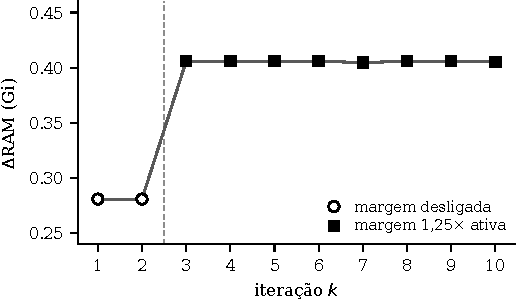
\includegraphics[width=\linewidth]{figuras/fig_exp01_delta_ram.pdf}
  \fonte{Elaborado pelo autor (2026).}
\end{figure}

\subsection{Experimento 2: seleção com um nó sobrecarregado}

O estresse foi efetivo: após o aquecimento, o \textit{worker} \textit{fog}
apresentou $1783$\,m de CPU contra cerca de $20$\,m nos
demais. A submissão direta atribuiu $2/5$ tarefas ao nó sobrecarregado,
enquanto o \textit{broker} não atribuiu nenhuma (Tabela~\ref{tab:exp02} e
Figura~\ref{fig:exp02}). As cinco tarefas do \textit{broker} foram para o
\texttt{worker3} (\textit{cloud}), embora a preferência registrada fosse
\textit{fog}, ou seja, o critério de recursos superou a preferência de camada, o que
é coerente com o menor peso relativo da afinidade de acordo com a equação
\eqref{eq:noderanker}.

\begin{table}[h]
  \caption{Experimento 2: posicionamento das cinco tarefas.}
  \label{tab:exp02}
  \centering\footnotesize
  \begin{tabular}{@{}cllcl@{}}
    \toprule
    $i$ & Direta & Sobrec. & \textit{Broker} & $t_{\mathrm{c}}$ (s)\\
    \midrule
    1 & \texttt{worker3} & não & \texttt{worker3} & $94{,}52$\\
    2 & \texttt{worker2} & sim & \texttt{worker3} & $95{,}32$\\
    3 & \texttt{worker3} & não & \texttt{worker3} & $98{,}74$\\
    4 & \texttt{worker2} & sim & \texttt{worker3} & $92{,}53$\\
    5 & \texttt{worker}  & não & \texttt{worker3} & $94{,}30$\\
    \bottomrule
  \end{tabular}
  \nota{$t_{\mathrm{c}}$: duração do contêiner no \textit{broker}. Os nós
  \texttt{worker}, \texttt{worker2} e \texttt{worker3} correspondem às camadas
  \textit{edge}, \textit{fog} e \textit{cloud}.}
  \fonte{Elaborado pelo autor (2026).}
\end{table}

\begin{figure}[t]
  \caption{Experimento 2: Jobs alocados por nó.}
  \label{fig:exp02}
  \centering
  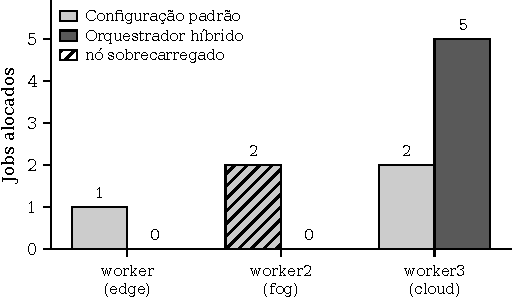
\includegraphics[width=\linewidth]{figuras/fig_exp02_placement.pdf}
  \fonte{Elaborado pelo autor (2026).}
\end{figure}

\subsection{Experimento 3: admissão \textit{best-effort}}

Este experimento verifica o mecanismo descrito na Seção~\ref{sec:metodos}:
uma requisição maior que a capacidade de qualquer nó, mas dentro da janela
de $80\%$, deve ser reduzida e executada, e não ficar parada na fila. Os dois
modelos solicitaram exatamente \gi{9,45} (\mi{9676}), o que isola o
efeito do mecanismo de admissão. Na submissão direta, a requisição
permaneceu sem nó durante os $90$\,s de monitoramento ($18$ amostras sem nome
de nó), com o evento de falha de escalonamento \textit{"0/4 nodes are
available"}, um nó por restrição do plano de controle e três por memória
insuficiente, apesar de cada \textit{worker} ter \gi{7,716} alocáveis. No
\textit{broker}, com capacidade efetiva máxima $R_{\max}=\gi{7,567}$ e teto
da janela em \gi{9,459}, a requisição foi reduzida para \mi{7748}
(\gi{7,57}), registrada como admissão \textit{best-effort}, e o Job foi
concluído no \texttt{worker2}, em $123{,}98$\,s totais, dos quais $74{,}97$\,s
de execução. O \textit{broker} usou a imagem
\texttt{python:3.9-slim} e a linha de base, \texttt{python:3.11-slim}; como a
admissão depende só de CPU e memória, a diferença não afeta a conclusão.
A requisição de \gi{9,45} ficou logo abaixo do teto da janela
(\gi{9,459}); portanto, o experimento testa o caso limite da regra e não um
caso intermediário. Pedidos acima desse teto permaneceriam na fila por
projeto. O resultado mostra que a regra evita o Pod sem nó, mas não mede o
efeito da redução de \gi{9,45} para \gi{7,57} (cerca de $20\%$) sobre o
desempenho da tarefa.

\subsection{Experimento 4: camada preferida versus camada alocada}\label{sec:exp04}

Em nove tarefas, o \textit{broker} obteve $4/9$ correspondências exatas de
camada ($44{,}4\%$) contra $1/9$ da submissão direta ($11{,}1\%$), e $9/9$
de correspondência adjacente (Figura~\ref{fig:exp04}). A camada preferida,
derivada do perfil produzido pelo LLM, foi \textit{fog} ou \textit{cloud} em
todas as tarefas, nenhuma \textit{edge}; o acerto foi de $1/3$ para
\textit{fog} e $3/6$ para \textit{cloud}, e as alocações ficaram em
\textit{cloud} ($5$) e \textit{fog} ($4$). A concordância entre essa
preferência e a camada nominal de cada \textit{script} foi de $3/9$, todas
em \textit{cloud}. A divergência em relação à camada nominal não foi
isolada; como o Analista, isolado, produziu a mesma saída em dez repetições
com temperatura zero (Seção~\ref{sec:temperatura}), a hipótese mais
provável é que a preferência de camada tenha dependido dos recursos
dimensionados a partir do histórico, e não da amostragem do LLM.

\begin{figure}[t]
  \caption{Experimento 4: camada preferida versus camada de execução.}
  \label{fig:exp04}
  \centering
  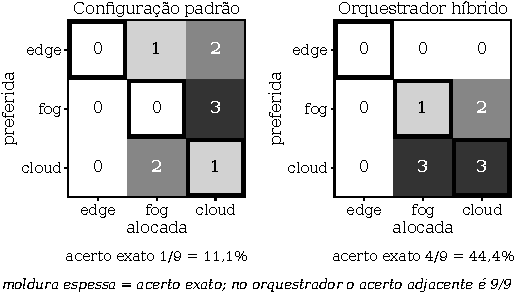
\includegraphics[width=\linewidth]{figuras/fig_exp04_matrizes.pdf}
  \fonte{Elaborado pelo autor (2026).}
\end{figure}

\subsection{Sensibilidade à temperatura do LLM}\label{sec:temperatura}

\begin{table}[h]
  \caption{Sensibilidade à temperatura: $40$ execuções por temperatura.}
  \label{tab:temperatura}
  \centering\footnotesize
  \setlength{\tabcolsep}{3pt}
  \begin{tabular}{@{}lccc@{}}
    \toprule
    Medida & $T=0$ & $T=0{,}5$ & $T=1{,}0$\\
    \midrule
    JSON do Analista válido & $40/40$ & $40/40$ & $40/40$\\
    Especificação válida & $40/40$ & $40/40$ & $40/40$\\
    Saídas distintas do Analista & 1/1/1/1 & 6/5/1/2 & 6/8/3/4\\
    Saídas distintas do Strategist & 1/1/1/1 & 2/3/2/3 & 5/4/6/5\\
    Desvio da complexidade (máx.) & $0$ & $0{,}77$ & $1{,}26$\\
    Tipo de tarefa alterado & $0$ & $1$ & $4$\\
    Camada preferida alterada & $0$ & $1$ & $4$\\
    \bottomrule
  \end{tabular}

  \fonte{Elaborado pelo autor (2026).}
\end{table}

Para verificar a escolha da temperatura, as respostas do Analista e do
Strategist foram comparadas em temperaturas $0$, $0{,}5$ e $1{,}0$, sem
executar tarefas no \textit{cluster}. Cada um dos quatro \textit{scripts} de
avaliação foi processado dez vezes por temperatura, com os mesmos prompts do \textit{broker}, o Librarian
em estado inicial (sem histórico) e sem fixar a semente do modelo, o que
totaliza $120$ execuções. A camada preferida foi calculada pela mesma regra
determinística do \textit{broker}, com os pisos iniciais de recursos. A
Tabela~\ref{tab:temperatura} resume os resultados.



Com temperatura zero, as dez repetições de cada \textit{script} produziram
exatamente a mesma saída do Analista e do Strategist, o que sustenta a
reprodutibilidade. O JSON e a especificação foram válidos em todas as
execuções nas três temperaturas, de modo que, neste modelo e nestes
\textit{scripts}, aumentar a temperatura não trouxe ganho de validade. O que
aumentou foi a variabilidade: com $T=1{,}0$ o Analista chegou a oito saídas
distintas em dez repetições para um mesmo \textit{script}. Em cinco
execuções com $T\geq 0{,}5$ a tarefa leve ou de memória foi reclassificada
como IO-bound, o que a levou à camada \textit{edge}; essas mudanças são
aleatórias e, no \textit{script} de CPU e no de aprendizado de máquina, a
camada preferida não mudou.

\subsection{Discussão}

\textbf{O que o LLM contribui.} No fluxo, o LLM converte o código em perfil e
em especificação estruturada, e o histórico recalibra o piso na execução
seguinte (Exp.~1). A escolha do nó e a admissão, porém, são determinísticas,
no Exp.~2 foi o NodeRanker, e no Exp.~3 a regra de $80\%$, que evitaram o nó
sob estresse e o Pod sem nó. A contribuição do LLM não foi avaliada de forma isolada, isto é, não se comparou o fluxo com uma heurística sem LLM; o que se
mostra é que o fluxo com LLM funciona e não está no caminho da
decisão crítica. Um modelo de cerca de $8$ bilhões de parâmetros foi testado
durante o desenvolvimento, mas gerou respostas longas e \textit{timeouts} ao
competir com o \textit{cluster} pelos mesmos recursos físicos, e por isso
adotou-se o modelo menor; trata-se de uma observação, não de uma comparação
controlada.

\textbf{Temperatura e preferência de camada.} A análise de sensibilidade
mostra que temperatura zero dá reprodutibilidade sem perda de validade, que
é o que a arquitetura exige de um componente que apenas propõe. Já a
baixa concordância ($3/9$) entre a preferência de camada e a camada nominal
no Exp.~4 não decorre da amostragem do Analista, que foi determinístico com
$T=0$, mas provavelmente dos recursos dimensionados a partir do histórico.
O acerto exato de $4/9$ depende da decisão final do nó, que independe do
LLM. Observa-se ainda que o perfil CPU-bound leva à camada
\textit{fog} pela regra de preferência, o que torna \textit{edge} rara; a
própria regra, e não só o LLM, limita essa preferência.

\textbf{Pesos e regra de admissão.} O resultado do Exp.~2, em que o critério
de recursos superou a preferência de camada, é compatível com a priorização
da execução adotada nos pesos, mas não valida os valores específicos
($40$/$25$/$15$/$20$). No Exp.~3, a regra só atua na janela de $80\%$,
requisições acima de $1{,}25R_{\max}$ permanecem na fila por projeto.

\subsection{Limitações e ameaças à validade}\label{sec:ameacas}

(i) Todos os experimentos executaram em um único hospedeiro, com camadas
lógicas; o Exp.~4 não permite concluir sobre latência ou desempenho de
infraestruturas \textit{Edge}, \textit{Fog} ou \textit{Cloud} físicas.
(ii) Os três \textit{workers} reportam \gi{7,716} alocáveis cada, porém
compartilham os \gi{15,9} físicos do hospedeiro, que também executa o LLM;
a capacidade é, portanto, nominal. (iii) As amostras são pequenas ($1$ a
$10$ execuções) e sem tratamento estatístico. (iv) A telemetria reflete o
momento da coleta e pode mudar entre a consulta e a execução, o que afeta
sobretudo o Exp.~2. (v) A sobrecarga do LLM na máquina compartilhada torna
os tempos ponta a ponta do \textit{broker} não comparáveis, como medida de
desempenho, com os da submissão direta. (vi) Não houve análise de
sensibilidade dos pesos; também não houve comparação experimental com outros
escalonadores. (vii) Em alguns casos o \textit{broker} usou
\texttt{python:3.9-slim} no lugar de \texttt{python:3.11-slim}.

%% ============================ 6 CONCLUSÃO ===================================
\section{Conclusão}\label{sec:conclusao}

Este trabalho propôs e avaliou um \textit{broker} externo ao plano de
controle do Kubernetes em que um LLM local interpreta a tarefa e propõe a
especificação, e regras determinísticas verificam a viabilidade, admitem a
requisição e escolhem o nó. Nos cenários avaliados, a abordagem recalibrou o
piso de recursos a partir do histórico (a margem de $1{,}25\times$ foi
ativada a partir da terceira execução), evitou o nó sob estresse nas cinco
tarefas, reduziu uma requisição de \gi{9,45} para \gi{7,57} e a executou,
enquanto a submissão direta permaneceu sem nó, e elevou o acerto exato de
camada de $1/9$ para $4/9$. O objetivo geral foi atendido no escopo
avaliado, e cada objetivo específico tem evidência correspondente: (a) a
arquitetura separa as funções do LLM das decisões determinísticas
(Quadro~\ref{qua:papeis}); (b) o NodeRanker e a admissão \textit{best-effort}
foram implementados e atuaram nos Exp.~2 e 3; (c) os quatro experimentos
foram executados e comparados à submissão direta; e (d) os \textit{logs} de
cada execução foram preservados.

As principais limitações são o ambiente em um único hospedeiro, as amostras
pequenas, os pesos definidos manualmente e a ausência de ablação do LLM; os
resultados constituem uma validação inicial e não demonstram otimização
global nem superioridade sobre o escalonador nativo.

Como trabalhos futuros, propõe-se: (i) a condução de um conjunto padronizado de testes (\textit{benchmark}) com cargas heterogêneas (CPU, E/S e aprendizado de máquina), repetições suficientes para tratamento estatístico e métricas consolidadas (tempo em \textit{Pending}, $\Delta$RAM, estrangulamento, acerto de camada e variância entre execuções), executado em infraestrutura fisicamente distribuída e comparado a outras abordagens de referência; (ii) a análise de sensibilidade dos pesos do NodeRanker e a avaliação da temperatura de amostragem com diferentes modelos e maior número de repetições, aplicadas também diretamente no \textit{cluster}; (iii) a avaliação isolada da contribuição do LLM frente a uma heurística tradicional sem modelo de linguagem; e (iv) a incorporação de modelos preditivos baseados em séries históricas para o dimensionamento automático de CPU e memória.

%% ========================= ELEMENTOS PÓS-TEXTUAIS ==========================
\bibliography{referencias}

\section*{Agradecimentos}

Agradeço à Universidade Tecnológica Federal do Paraná (UTFPR), Câmpus Apucarana, pelo suporte institucional, e ao Prof. André Luiz Tinassi D'Amato pela orientação e pelo rigor metodológico na condução desta pesquisa. Agradeço, ainda, aos meus familiares e amigos pelo incentivo e apoio durante toda a graduação.

\end{document}
